\documentclass[11pt,a4paper]{article}

% ================= Encodage & langue =================
\usepackage[utf8]{inputenc}
\usepackage[T1]{fontenc}
\usepackage[french]{babel}
\usepackage{lmodern}
\usepackage{microtype}

% ================= Mise en page =================
\usepackage[margin=2.4cm]{geometry}
\usepackage{setspace}
\usepackage{parskip}
\setstretch{1.1}

% ================= Couleurs & liens =================
\usepackage{xcolor}
\definecolor{udemblue}{HTML}{0B3D91}
\definecolor{codegray}{HTML}{F4F4F4}
\definecolor{keyword}{HTML}{0057B7}
\definecolor{comment}{HTML}{6A737D}
\definecolor{string}{HTML}{B8860B}

\usepackage[colorlinks=true, linkcolor=udemblue, urlcolor=udemblue,
            citecolor=udemblue]{hyperref}

% ================= Titres =================
\usepackage{titlesec}
\titleformat{\section}
  {\color{udemblue}\Large\bfseries}{\thesection}{0.7em}{}
\titleformat{\subsection}
  {\color{udemblue}\large\bfseries}{\thesubsection}{0.6em}{}
\titleformat{\subsubsection}
  {\normalsize\bfseries}{\thesubsubsection}{0.5em}{}

% ================= Tableaux & figures =================
\usepackage{booktabs}
\usepackage{array}
\usepackage{tabularx}
\usepackage{longtable}
\usepackage{graphicx}
\usepackage{float}
\usepackage{caption}
\captionsetup{font=small, labelfont={bf,color=udemblue}}

% ================= Listings SQL / C# =================
\usepackage{listings}
\lstdefinelanguage{TSQL}{
  morekeywords={SELECT,FROM,WHERE,JOIN,LEFT,RIGHT,INNER,OUTER,ON,GROUP,BY,
    ORDER,HAVING,AS,AND,OR,NOT,NULL,IS,IN,EXISTS,CREATE,TABLE,VIEW,TRIGGER,
    FUNCTION,PROCEDURE,RETURN,RETURNS,BEGIN,END,DECLARE,SET,INSERT,INTO,
    VALUES,UPDATE,DELETE,ALTER,DROP,CONSTRAINT,PRIMARY,KEY,FOREIGN,REFERENCES,
    UNIQUE,CHECK,DEFAULT,IDENTITY,INT,VARCHAR,DATE,DECIMAL,BIT,CAST,CONVERT,
    GETDATE,COUNT,SUM,AVG,MIN,MAX,NULLIF,ISNULL,COALESCE,IF,ELSE,WHILE,
    CURSOR,OPEN,FETCH,CLOSE,DEALLOCATE,NEXT,AFTER,INSTEAD,OF,OUTER,APPLY,
    USE,GO,EXEC,OUTPUT,ROLLBACK,COMMIT,TRANSACTION,RAISERROR,THROW,TRY,CATCH,
    PRINT,CONCAT,ROUND,TOP,DISTINCT,UNION,LIKE,BETWEEN,CASE,WHEN,THEN,ELSE},
  sensitive=false,
  morecomment=[l]{--},
  morecomment=[s]{/*}{*/},
  morestring=[b]'
}
\lstset{
  basicstyle=\ttfamily\footnotesize,
  keywordstyle=\color{keyword}\bfseries,
  commentstyle=\color{comment}\itshape,
  stringstyle=\color{string},
  backgroundcolor=\color{codegray},
  frame=single,
  rulecolor=\color{codegray},
  breaklines=true,
  breakatwhitespace=true,
  showstringspaces=false,
  columns=fullflexible,
  numbers=left,
  numberstyle=\tiny\color{comment},
  numbersep=6pt,
  xleftmargin=1.5em,
  captionpos=b,
  language=TSQL,
  extendedchars=true,
  literate=
    {é}{{\'e}}1 {è}{{\`e}}1 {ê}{{\^e}}1 {ë}{{\"e}}1
    {à}{{\`a}}1 {â}{{\^a}}1 {ä}{{\"a}}1
    {ô}{{\^o}}1 {ö}{{\"o}}1
    {î}{{\^i}}1 {ï}{{\"i}}1
    {ù}{{\`u}}1 {û}{{\^u}}1 {ü}{{\"u}}1
    {ç}{{\c{c}}}1 {É}{{\'E}}1 {È}{{\`E}}1 {Ê}{{\^E}}1
    {À}{{\`A}}1 {Â}{{\^A}}1 {Ç}{{\c{C}}}1
    {«}{{\guillemotleft}}1 {»}{{\guillemotright}}1
    {œ}{{\oe}}1 {°}{{\textdegree}}1 {’}{{'}}1
}

% ================= Variables (à remplacer au besoin) =================
\newcommand{\matEdouard}{XXXXXXXX}
\newcommand{\matFlorion}{XXXXXXXX}
\newcommand{\matGaius}{XXXXXXXX}
\newcommand{\matImad}{XXXXXXXX}

% ================= Document =================
\begin{document}

% ================= Page de garde =================
\begin{titlepage}
    \centering
    \vspace*{1.5cm}

    {\scshape\Large Université de Montréal \par}
    \vspace{0.3cm}
    {\scshape\large Faculté des arts et des sciences --- Département d'informatique \par}
    \vspace{0.2cm}
    {\scshape IFT 2821 --- Bases de données \par}

    \vspace{2.5cm}
    {\color{udemblue}\rule{\linewidth}{0.6mm}}
    \vspace{0.6cm}

    {\Huge\bfseries Projet de session\par}
    \vspace{0.5cm}
    {\LARGE Gestion des inscriptions et des notes\\dans une université\par}

    \vspace{0.5cm}
    {\color{udemblue}\rule{\linewidth}{0.6mm}}

    \vspace{2cm}
    
    \begin{tabular}{ll}
        \textbf{Édouard Bibeau}                  & 20247400 \\
        \textbf{Florion-Victor Buhendwa Chalazire} & 20364625 \\
        \textbf{Gaius Heumen Nkouantchoua}        & \matGaius   \\
        \textbf{Imad Baida}                       & 20363685      \\
    \end{tabular}

    \vfill

    {\large Travail présenté à\\[0.2cm]\textbf{Jihen Rezgui}\par}
    \vspace{0.8cm}
    {\large 16 avril 2026\par}
\end{titlepage}

\tableofcontents
\newpage


% =====================================================================
\section{Introduction et reformulation du cahier des charges}
% =====================================================================

Le but du projet est de concevoir et implanter une base de données pour
gérer les inscriptions et les notes dans une université, en SQL Server.
On veut couvrir tout le parcours d'un étudiant : de son admission dans
un programme jusqu'à sa note finale dans un cours, en passant par
l'offre de cours par semestre, les sessions d'examen et l'administration
des profs.

\subsection{Reformulation}

L'énoncé donne six grands blocs d'information. Voici comment on les a
interprétés avant de faire le modèle :

\begin{description}
    \item[Acteurs.] Il y a trois types d'utilisateurs : les étudiants,
        les professeurs et les administrateurs. Comme ils partagent
        beaucoup d'information (nom, prénom, courriel, téléphone,
        adresse), on a choisi de tout mettre dans une seule entité
        \texttt{Utilisateur} et de faire hériter les trois rôles via une
        relation 1--1. Ça évite d'avoir la même info dupliquée dans
        trois tables différentes.
    \item[Programmes et spécialisations.] Chaque étudiant fait au plus
        un programme à la fois. Dans son programme, il peut choisir une
        ou plusieurs spécialisations (un peu comme une majeure/mineure),
        donc on a fait une association n--m avec \texttt{ChoixSpecialisation}
        pour garder la date et l'ordre des choix.
    \item[Catalogue de cours.] Un cours a un code unique, un type
        (théorique, labo, TP, démo) et un nombre de crédits. Comme un
        cours peut appartenir à plusieurs programmes, on passe par
        \texttt{CoursProgramme}. Pour les prérequis on a fait une
        association réflexive \texttt{CoursPrerequis}, vu qu'un prérequis
        est lui-même un cours. Enfin, une spécialisation peut réserver
        des places sur certains cours, c'est géré par \texttt{Restreindre}.
    \item[Sections et horaires.] L'énoncé dit qu'un cours peut être
        divisé en sections avec des horaires différents. On a donc
        séparé le cours « catalogue » de son instance concrète dans un
        semestre : c'est la table \texttt{CoursOffert}
        (section, salle, horaire, capacité, mode d'enseignement).
    \item[Semestres et sessions d'examen.] L'année universitaire est
        divisée en semestres (Hiver, Été, Automne d'une année donnée).
        Chaque semestre a une ou plusieurs sessions d'examen (intra,
        final, reprise, etc.) regroupées dans \texttt{SessionExamen}.
    \item[Évaluations et notes.] Dans un cours offert on peut avoir
        plusieurs évaluations (TP, quiz, intra, examen final), chacune
        avec son poids. La note d'un étudiant à une évaluation va dans
        la table \texttt{Note}, qui est liée à son inscription au cours.
    \item[Inscription et historique.] L'inscription d'un étudiant à un
        cours offert est représentée par \texttt{Inscription} : date,
        statut (inscrit, annulé), note finale, décision (réussi, échec,
        abandon), numéro de tentative et validation des prérequis.
\end{description}

\subsection{Justification des choix de conception}

\begin{itemize}
    \item \textbf{Identifiants entiers \texttt{IDENTITY}} plutôt que
        des codes textuels : ça rend les jointures plus simples et on
        garde quand même un champ \texttt{code\_*} lisible quand c'est
        utile (cours, programme).
    \item \textbf{Colonne calculée \texttt{mat\_User}} : c'est le
        matricule sur 10 chiffres (AAAAMMXXXX) construit automatiquement
        à partir de l'année et du mois d'inscription et de l'id. Comme
        ça on n'a pas à le saisir à la main et il reste toujours
        cohérent avec les autres champs.
    \item \textbf{Héritage \texttt{Utilisateur} vers \texttt{Etudiant},
        \texttt{Professeur}, \texttt{Administrateur}} : un même courriel
        ne peut pas appartenir à deux personnes, et un utilisateur peut
        devenir prof ou admin sans devoir recréer ses infos.
    \item \textbf{\texttt{Cours} séparé de \texttt{CoursOffert}} : le
        cours dans le catalogue et le cours offert dans un semestre
        donné ne sont pas la même chose. C'est ce qui permet à un
        étudiant de reprendre IFT2821 en hiver 2026 après l'avoir
        échoué en automne 2025.
    \item \textbf{CHECK et UNIQUE} : format du téléphone et du courriel,
        liste fermée pour les types de cours, d'évaluation et les
        grades, et surtout \texttt{UNIQUE(id\_Etud, id\_CoursOf)} pour
        empêcher la double inscription au même cours. Les lettres de
        notes sont aussi restreintes au barème UdeM
        (A+, A, A-, B+, B, B-, C+, C, C-, D+, D, E, F).
\end{itemize}


% =====================================================================
\section{Modèle entité-association}
% =====================================================================

Le modèle contient dix entités principales plus cinq associations qu'on
a nommées parce qu'elles portent des attributs (comme la date du choix,
le nombre de places, etc.).

\subsection{Entités et attributs}

\begin{longtable}{@{}p{3.4cm} p{11.8cm}@{}}
\toprule
\textbf{Entité} & \textbf{Attributs (identifiant souligné)} \\
\midrule
\endfirsthead
\toprule
\textbf{Entité} & \textbf{Attributs (identifiant souligné)} \\
\midrule
\endhead

Utilisateur &
    \underline{id\_User}, nom\_User, prenom\_User, dateInscriptUser,
    mat\_User, dateNais\_User, numTel\_User, courriel\_User,
    passwordHash\_User, adresse\_User \\

Etudiant (is-a Utilisateur) &
    \underline{id\_User}, statut\_Etud, programme\_Etud \\

Professeur (is-a Utilisateur) &
    \underline{id\_User}, grade\_Prof, statut\_Prof \\

Administrateur (is-a Utilisateur) &
    \underline{id\_User}, role\_Admin\_Etud \\

Programme &
    \underline{id\_Prog}, code\_Prog, nom\_Prog, descript\_Prog,
    nbCredit\_Prog, unite\_Prog, duree\_Prog, dateCreat\_Prog \\

Specialisation &
    \underline{id\_Spec}, nom\_Spec, descript\_Spec, nbCredit\_Spec \\

Cours &
    \underline{id\_Cours}, code\_Cours, nom\_Cours, credit\_Cours,
    type\_Cours, nbHeure\_Cours \\

CoursOffert &
    \underline{id\_CoursOf}, sect\_CoursOf, capacite\_CoursOf,
    horaire\_CoursOf, salle\_CoursOf, dateDeb\_CoursOf, dateFin\_CoursOf,
    mondeEns\_CoursOf \\

Semestre &
    \underline{id\_Semest}, nom\_Semest, annee\_Semest,
    datDeb\_Semest, dateFin\_Semest \\

SessionExamen &
    \underline{id\_SessExam}, type\_SessExam, dateDeb, dateFin \\

Evaluation &
    \underline{id\_Eval}, type\_Eval, date\_Eval, nom\_Eval,
    poids\_Eval, descript\_Eval \\

Inscription (association) &
    \underline{id\_Inscript}, statut\_Inscript, date\_Inscript,
    date\_Desinscript, noteFi\_Inscript, noteLet\_Inscript,
    decisionFi\_Inscript, tentative\_Inscript,
    estValidePrerequis\_Inscript \\

Note (association) &
    \underline{id\_Note}, valNum\_Note, ValLettre\_Note, retroAction,
    dateAttrib\_Note \\

Enseigner (association) &
    \underline{id\_Enseigner}, nbH\_Enseigner, datDeb\_Enseigner,
    dateFin\_Enseigner \\

ChoixSpecialisation (association) &
    \underline{id\_ChoixSpec}, date\_ChoixSpec, nb\_ChoixSpec \\

Restreindre (association) &
    \underline{id\_Rest}, nb\_Restrict \\

\bottomrule
\end{longtable}

\subsection{Associations et cardinalités}

\begin{longtable}{@{}p{5.3cm} p{3.2cm} p{6.6cm}@{}}
\toprule
\textbf{Association} & \textbf{Cardinalité} & \textbf{Sémantique} \\
\midrule
\endhead

Etudiant --- Programme                & 0,n --- 1,1   & Un étudiant appartient à au plus un programme. \\
Specialisation --- Programme          & 0,n --- 1,1   & Une spécialisation appartient à un programme. \\
ChoixSpecialisation (Etudiant, Specialisation) & n --- m & Un étudiant peut choisir plusieurs spécialisations. \\
CoursProgramme (Cours, Programme)     & n --- m       & Un cours peut appartenir à plusieurs programmes. \\
CoursPrerequis (Cours, Cours)         & n --- m (réflexive) & Un cours peut avoir plusieurs prérequis. \\
Restreindre (Specialisation, Cours)   & n --- m       & Réservation de places par spécialisation. \\
CoursOffert --- Cours                 & 0,n --- 1,1   & Une offre concrétise un cours du catalogue. \\
CoursOffert --- Semestre              & 0,n --- 1,1   & L'offre est située dans un semestre. \\
Inscription (Etudiant, CoursOffert)   & n --- m       & Unique par couple (contrainte \texttt{UNIQUE}). \\
Enseigner (Professeur, CoursOffert)   & n --- m       & Un cours offert peut avoir plusieurs professeurs. \\
SessionExamen --- Semestre            & 0,n --- 1,1   & Une session est rattachée à un semestre. \\
Evaluation --- CoursOffert            & 0,n --- 1,1   & Une évaluation appartient à un cours offert. \\
Evaluation --- SessionExamen          & 0,n --- 1,1   & Une évaluation se tient dans une session. \\
Note --- Inscription                  & 0,n --- 1,1   & Une note concerne une inscription précise. \\
Note --- Evaluation                   & 0,n --- 1,1   & Une note porte sur une évaluation précise. \\

\bottomrule
\end{longtable}

\begin{figure}[H]
    \centering
    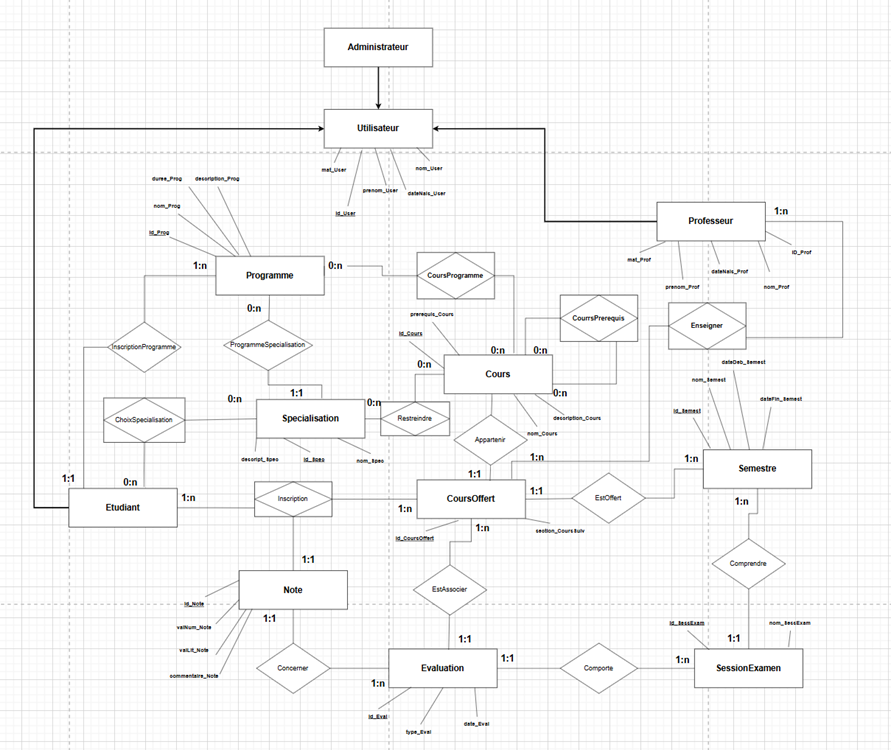
\includegraphics[width=\linewidth]{figures/schema_entite_association}
    \caption{Schéma entité-association de la base
        \texttt{GestionInscriptEtudiant}.}
    \label{fig:schema-ea}
\end{figure}


% =====================================================================
\section{Modèle relationnel}
% =====================================================================

La transformation du schéma E-A donne dix-sept relations. Les clés
primaires sont \underline{soulignées} et les clés étrangères préfixées
par un \texttt{\#}.

\begin{itemize}\small
    \item \texttt{Programme(\underline{id\_Prog}, code\_Prog, nom\_Prog,
        descript\_Prog, nbCredit\_Prog, unite\_Prog, duree\_Prog,
        dateCreat\_Prog)}

    \item \texttt{Specialisation(\underline{id\_Spec}, nom\_Spec,
        descript\_Spec, nbCredit\_Spec, \#id\_Prog\_Spec)}

    \item \texttt{Utilisateur(\underline{id\_User}, nom\_User, prenom\_User,
        dateInscriptUser, mat\_User, dateNais\_User, numTel\_User,
        courriel\_User, passwordHash\_User, adresse\_User)}

    \item \texttt{Etudiant(\underline{\#id\_User}, statut\_Etud,
        \#programme\_Etud)}

    \item \texttt{Professeur(\underline{\#id\_User}, grade\_Prof,
        statut\_Prof)}

    \item \texttt{Administrateur(\underline{\#id\_User},
        role\_Admin\_Etud)}

    \item \texttt{Cours(\underline{id\_Cours}, code\_Cours, nom\_Cours,
        credit\_Cours, type\_Cours, nbHeure\_Cours)}

    \item \texttt{CoursProgramme(\underline{id\_CoursProg}, \#id\_Prog,
        \#id\_Cours)}

    \item \texttt{CoursPrerequis(\underline{id\_CoursPre}, \#id\_Cours,
        \#id\_Prerequis)}

    \item \texttt{Semestre(\underline{id\_Semest}, nom\_Semest,
        annee\_Semest, datDeb\_Semest, dateFin\_Semest)}

    \item \texttt{CoursOffert(\underline{id\_CoursOf}, sect\_CoursOf,
        capacite\_CoursOf, horaire\_CoursOf, salle\_CoursOf,
        dateDeb\_CoursOf, dateFin\_CoursOf, mondeEns\_CoursOf,
        \#id\_Cours, \#id\_Semest)}

    \item \texttt{SessionExamen(\underline{id\_SessExam}, type\_SessExam,
        dateDeb, dateFin, \#id\_Semest)}

    \item \texttt{Evaluation(\underline{id\_Eval}, type\_Eval, date\_Eval,
        nom\_Eval, poids\_Eval, descript\_Eval, \#id\_CoursOf,
        \#id\_SessExam)}

    \item \texttt{ChoixSpecialisation(\underline{id\_ChoixSpec},
        date\_ChoixSpec, nb\_ChoixSpec, \#id\_Etud, \#id\_Spec)}

    \item \texttt{Inscription(\underline{id\_Inscript}, statut\_Inscript,
        date\_Inscript, date\_Desinscript, noteFi\_Inscript,
        noteLet\_Inscript, decisionFi\_Inscript, tentative\_Inscript,
        estValidePrerequis\_Inscript, \#id\_Etud, \#id\_CoursOf)}

    \item \texttt{Note(\underline{id\_Note}, valNum\_Note, ValLettre\_Note,
        retroAction, dateAttrib\_Note, \#id\_Inscript, \#id\_Eval)}

    \item \texttt{Restreindre(\underline{id\_Rest}, nb\_Restrict,
        \#id\_Spec, \#id\_Cours)}

    \item \texttt{Enseigner(\underline{id\_Enseigner}, nbH\_Enseigner,
        datDeb\_Enseigner, dateFin\_Enseigner, \#id\_Prof,
        \#id\_CoursOf)}
\end{itemize}


% =====================================================================
\section{Normalisation}
% =====================================================================

\subsection{Première forme normale (1FN)}

Pour être en 1FN il faut que tous les attributs soient atomiques (pas
de liste, pas d'attribut multi-valué) et que chaque ligne soit
identifiable de façon unique. Dans nos tables on a tout décomposé en
champs simples (l'adresse, les noms, etc.) et chaque table a sa propre
clé primaire, donc la 1FN est respectée partout.

\subsection{Deuxième forme normale (2FN)}

Pour être en 2FN il faut déjà être en 1FN, et qu'aucun attribut non-clé
ne dépende seulement d'une partie de la clé primaire. Chez nous toutes
les clés primaires sont simples (un seul id auto-incrémenté), donc on
ne peut pas avoir de dépendance partielle : la 2FN est respectée
automatiquement.

Les principales dépendances fonctionnelles sont :
\begin{center}\small
\begin{tabular}{@{}ll@{}}
\toprule
\textbf{Déterminant} & \textbf{Déterminés} \\
\midrule
id\_User      & nom\_User, prenom\_User, dateNais\_User, \ldots, mat\_User \\
id\_Prog      & code\_Prog, nom\_Prog, nbCredit\_Prog, \ldots \\
id\_Cours     & code\_Cours, nom\_Cours, credit\_Cours, type\_Cours, \ldots \\
id\_CoursOf   & sect, capacite, horaire, salle, \#id\_Cours, \#id\_Semest \\
id\_Eval      & type, date, nom, poids, \#id\_CoursOf, \#id\_SessExam \\
id\_Inscript  & statut, dates, noteFi, noteLet, \#id\_Etud, \#id\_CoursOf \\
id\_Note      & valNum, valLettre, retroAction, \#id\_Inscript, \#id\_Eval \\
\bottomrule
\end{tabular}
\end{center}

\subsection{Troisième forme normale (3FN)}

La 3FN ajoute la condition qu'aucun attribut non-clé ne dépend d'un
autre attribut non-clé (pas de dépendance transitive). En regardant
nos DF ligne par ligne, toutes nos tables sont en 3FN.

Il y a par contre deux cas limites qu'on a identifiés et qu'on assume :

\begin{enumerate}
    \item \textbf{Table \texttt{Utilisateur}} :
        \texttt{id\_User $\to$ dateInscriptUser $\to$ mat\_User}. En
        théorie c'est une dépendance transitive, mais \texttt{mat\_User}
        est une colonne calculée et persistée (PERSISTED) par SQL
        Server à partir de la date et de l'id. Elle ne peut jamais être
        incohérente, donc on l'a gardée.

    \item \textbf{Table \texttt{Inscription}} :
        \texttt{id\_Inscript $\to$ noteFi\_Inscript $\to$ decisionFi\_Inscript}.
        La décision finale (Réussi, Échec, Abandon) pourrait se déduire
        de la note, mais on l'a stockée explicitement pour deux raisons.
        D'abord, le cas « Abandon » ne se déduit pas d'une note. Ensuite,
        la décision peut résulter d'un processus administratif (appel,
        reprise) qui n'est pas juste une question de seuil. Le trigger
        \texttt{trg\_Note\_RecalculerInscription} garde quand même
        cette colonne synchronisée automatiquement avec la moyenne.
\end{enumerate}


% =====================================================================
\section{Implantation SQL}
% =====================================================================

\subsection{LDD --- création des tables}

Le fichier \texttt{database/LDD\_LMD.sql} crée la base
\texttt{GestionInscriptEtudiant}, les 17 tables avec leurs contraintes
(PK, FK, CHECK, UNIQUE, DEFAULT), puis insère environ 190 lignes de
données de test réparties sur toutes les tables.

\begin{lstlisting}[caption={Extrait de \texttt{LDD\_LMD.sql} --- table Utilisateur}]
CREATE TABLE Utilisateur (
    id_User INT IDENTITY(100, 1),
    nom_User VARCHAR(50) NOT NULL,
    prenom_User VARCHAR(50) NOT NULL,
    dateInscriptUser DATE NOT NULL DEFAULT GETDATE(),
    mat_User AS (CAST(YEAR(dateInscriptUser) AS VARCHAR(4)) +
        RIGHT('00' + CAST(MONTH(dateInscriptUser) AS VARCHAR(2)), 2) +
        RIGHT('0000' + CAST(id_User AS VARCHAR(4)), 4)) PERSISTED UNIQUE,
    dateNais_User DATE NOT NULL,
    numTel_User VARCHAR(20) CHECK (numTel_User IS NULL OR
        numTel_User LIKE '[1-9][0-9][0-9][0-9][0-9][0-9][0-9][0-9][0-9][0-9]'),
    courriel_User VARCHAR(100) CHECK (courriel_User LIKE '%_@_%._%'),
    passwordHash_User VARCHAR(MAX),
    adresse_User VARCHAR(200),
    CONSTRAINT PK_Utilisateur PRIMARY KEY(id_User),
    CONSTRAINT UQ_Utilisateur_courriel UNIQUE(courriel_User)
);
\end{lstlisting}

\subsection{Requêtes SQL}

Le fichier \texttt{database/requetes.sql} contient :

\begin{itemize}
    \item \textbf{5 requêtes simples} (R1 à R5) : lister les notes, les
        cours restreints par spécialisation, les affectations prof-cours,
        le total d'heures par professeur, et les moyennes par évaluation.
    \item \textbf{5 requêtes complexes} (R6 à R10), toutes avec au moins
        4 tables jointes :
        \begin{enumerate}
            \item[R6.] Bulletin complet d'un étudiant (7 tables).
            \item[R7.] Moyenne pondérée par étudiant et par cours (6).
            \item[R8.] Liste des profs avec leurs cours et le programme
                associé (7).
            \item[R9.] Cours restreints par spécialisation avec le
                programme parent (6).
            \item[R10.] Résumé d'une session d'examen avec le prof
                responsable et la moyenne obtenue (8).
        \end{enumerate}
\end{itemize}

\begin{lstlisting}[caption={Exemple --- R7 : moyenne pondérée par étudiant et par cours}]
SELECT U.mat_User, U.nom_User, U.prenom_User,
       C.code_Cours, C.nom_Cours,
       ROUND(SUM(N.valNum_Note * Ev.poids_Eval) /
             NULLIF(SUM(Ev.poids_Eval), 0), 2) AS moyennePonderee
FROM Note N
JOIN Inscription I  ON N.id_Inscript = I.id_Inscript
JOIN Etudiant Et    ON I.id_Etud = Et.id_User
JOIN Utilisateur U  ON Et.id_User = U.id_User
JOIN Evaluation Ev  ON N.id_Eval = Ev.id_Eval
JOIN CoursOffert CO ON I.id_CoursOf = CO.id_CoursOf
JOIN Cours C        ON CO.id_Cours = C.id_Cours
GROUP BY U.mat_User, U.nom_User, U.prenom_User, C.code_Cours, C.nom_Cours;
\end{lstlisting}

\subsection{Transact-SQL}

Le fichier \texttt{database/T-SQL.sql} contient nos objets T-SQL :

\begin{description}
    \item[Fonctions.]
        \texttt{fn\_\allowbreak MoyennePondereeEtudiantCours} pour
        calculer la moyenne pondérée d'un étudiant dans un cours donné,
        \texttt{fn\_\allowbreak NoteLettre} qui applique le barème UdeM
        à une note sur 20, et \texttt{fn\_\allowbreak
        EtudiantsAuDessusMoyenne} qui retourne une table des étudiants
        ayant une moyenne supérieure à un seuil.
    \item[Procédures.]
        \texttt{sp\_\allowbreak InscrireEtudiantCours} qui fait
        l'inscription en vérifiant la capacité et les prérequis dans
        une transaction, \texttt{sp\_\allowbreak ReleveNotesEtudiant}
        qui génère le relevé de notes, et \texttt{sp\_\allowbreak
        MajNoteLettreInscription} qui utilise un \textbf{curseur} pour
        parcourir les inscriptions et mettre à jour les lettres
        manquantes.
    \item[Déclencheurs.]
        \texttt{trg\_\allowbreak Note\_\allowbreak RecalculerInscription}
        (AFTER INSERT/UPDATE/DELETE) recalcule la moyenne du cours et
        la lettre quand une note change,
        \texttt{trg\_\allowbreak Evaluation\_\allowbreak VerifierPoids}
        empêche la somme des poids des évaluations d'un cours de
        dépasser 100, et
        \texttt{trg\_\allowbreak Inscription\_\allowbreak
        EmpecherSuppression\allowbreak AvecNotes} (INSTEAD OF DELETE)
        bloque la suppression d'une inscription qui a déjà des notes.
    \item[Vue.]
        \texttt{v\_\allowbreak MoyenneFinaleEtudiant} donne la moyenne
        générale de chaque étudiant, tous cours confondus.
\end{description}

\begin{lstlisting}[caption={Extrait de \texttt{T-SQL.sql} --- déclencheur de recalcul}]
CREATE TRIGGER dbo.trg_Note_RecalculerInscription
ON  dbo.Note
AFTER INSERT, UPDATE, DELETE
AS
BEGIN
    SET NOCOUNT ON;
    DECLARE @inscriptions TABLE (id_Inscript INT PRIMARY KEY);
    INSERT INTO @inscriptions (id_Inscript)
    SELECT DISTINCT id_Inscript FROM inserted
    UNION
    SELECT DISTINCT id_Inscript FROM deleted;

    UPDATE I
    SET I.noteFi_Inscript    = X.moyenne,
        I.noteLet_Inscript   = dbo.fn_NoteLettre(X.moyenne),
        I.decisionFi_Inscript =
            CASE WHEN X.moyenne IS NULL THEN I.decisionFi_Inscript
                 WHEN X.moyenne >= 10   THEN 'Réussi'
                 ELSE 'Échec' END
    FROM Inscription I
    JOIN @inscriptions A ON I.id_Inscript = A.id_Inscript
    OUTER APPLY (
        SELECT CAST(SUM(N.valNum_Note * Ev.poids_Eval) /
                    NULLIF(SUM(Ev.poids_Eval), 0) AS DECIMAL(5,2)) AS moyenne
        FROM Note N
        JOIN Evaluation Ev ON N.id_Eval = Ev.id_Eval
        WHERE N.id_Inscript = I.id_Inscript
    ) AS X;
END;
\end{lstlisting}


% =====================================================================
\section{Application web}
% =====================================================================

On a fait l'application en ASP.NET Core Razor Pages (.NET 10). Pour
parler avec SQL Server on utilise Entity Framework Core, et pour les
mots de passe on utilise BCrypt. L'app exécute bien plus que les dix
instructions SQL demandées : chaque page de dashboard, d'inscription
ou de saisie de notes fait plusieurs requêtes pour charger et mettre
à jour les données.

\subsection{Architecture et rôles}

On a trois rôles gérés par authentification par cookies :
Administrateur, Professeur et Étudiant. Chaque page est protégée par
une politique d'autorisation (\texttt{AdminOnly},
\texttt{ProfesseurOnly}, \texttt{EtudiantOnly}) via l'attribut
\texttt{[Authorize]}.

\subsection{Fonctionnalités principales}

\begin{itemize}
    \item \textbf{Authentification.} Inscription, connexion,
        déconnexion, hachage BCrypt des mots de passe, et attribution
        automatique du rôle au moment de la connexion.
    \item \textbf{Étudiant.} Tableau de bord avec le dossier, les choix
        de spécialisation et les notes par cours. Page d'inscription
        qui filtre les cours selon le programme et vérifie la capacité,
        plus la possibilité de se désinscrire.
    \item \textbf{Professeur.} Liste des cours enseignés avec les
        étudiants inscrits, et un petit formulaire pour saisir la note
        finale. La note se rentre entre 0 et 20, la lettre est
        calculée automatiquement en JavaScript pendant la saisie, et
        la base valide le tout avec le trigger et le CHECK.
    \item \textbf{Administrateur.} Dashboard avec des stats
        (nombres d'étudiants, profs, cours, inscriptions), gestion des
        rôles et affectation des profs aux cours offerts.
\end{itemize}

\subsection{Intégration des objets T-SQL}

Plutôt que de tout faire en LINQ avec EF Core, on a branché quelques
endroits critiques directement sur nos objets T-SQL pour laisser le
SGBD faire son travail.

\begin{description}
    \item[\texttt{sp\_\allowbreak InscrireEtudiantCours}.]
        On l'appelle dans la page d'inscription de l'étudiant
        (\texttt{Pages/Etudiant/\allowbreak Inscription.cshtml.cs})
        chaque fois qu'un nouvel étudiant s'inscrit à un cours. La
        procédure vérifie la capacité, la non-duplication et les
        prérequis, le tout dans une transaction. Si la capacité est
        dépassée, le \texttt{RAISERROR} remonte jusqu'au code C\# qui
        attrape la \texttt{SqlException} et affiche le message à
        l'étudiant.
    \item[\texttt{v\_\allowbreak MoyenneFinaleEtudiant}.] On lit cette
        vue dans le dashboard admin (\texttt{AdminDashboard.cshtml.cs})
        avec \texttt{SqlQueryRaw<MoyenneEtudiantVue>} pour afficher le
        top 10 des moyennes.
    \item[Déploiement auto.] Au démarrage, \texttt{Program.cs} lit
        \texttt{T-SQL.sql} et l'exécute batch par batch. Comme le
        script utilise des \texttt{DROP IF EXISTS} avant chaque
        \texttt{CREATE}, il est idempotent, donc on n'a pas à y penser
        entre deux runs de l'application.
\end{description}

\subsection{Captures d'écran}

\begin{figure}[H]
    \centering
    \fbox{\parbox{0.9\linewidth}{\centering\vspace{1cm}
        \textit{(Page d'accueil / connexion)}\vspace{1cm}}}
    \caption{Page d'accueil et formulaire de connexion.}
\end{figure}

\begin{figure}[H]
    \centering
    \fbox{\parbox{0.9\linewidth}{\centering\vspace{1cm}
        \textit{(Tableau de bord étudiant)}\vspace{1cm}}}
    \caption{Tableau de bord de l'étudiant --- dossier, notes, inscriptions.}
\end{figure}

\begin{figure}[H]
    \centering
    \fbox{\parbox{0.9\linewidth}{\centering\vspace{1cm}
        \textit{(Saisie des notes côté professeur)}\vspace{1cm}}}
    \caption{Interface de saisie des notes par le professeur.}
\end{figure}

\begin{figure}[H]
    \centering
    \fbox{\parbox{0.9\linewidth}{\centering\vspace{1cm}
        \textit{(Tableau de bord administrateur)}\vspace{1cm}}}
    \caption{Tableau de bord de l'administrateur avec statistiques.}
\end{figure}


% =====================================================================
\section{Conclusion}
% =====================================================================

Dans ce projet on a couvert toutes les étapes demandées : le modèle
E-A avec 17 relations toutes en 3FN, la base SQL Server avec environ
190 tuples de test, 10 requêtes SQL (5 simples et 5 complexes à 4
tables ou plus), nos objets T-SQL (3 triggers, 3 fonctions, 3
procédures dont une avec un curseur, et une vue) et finalement une
application web en ASP.NET Core pour les trois rôles. En plus des
contraintes déclaratives (PK, FK, CHECK, UNIQUE), on utilise les
triggers pour garder la base cohérente dynamiquement : recalcul
automatique des moyennes, somme des poids d'évaluations qui ne peut
pas dépasser 100, et protection contre la suppression d'une
inscription qui aurait déjà des notes.

\end{document}
